\documentclass[border=10pt]{standalone}

\usepackage{tikz}
\usepackage{tikzsymbols}
\usetikzlibrary{calc,patterns,shapes.geometric}

\def\centerarc[#1](#2)(#3:#4:#5){\draw[#1] ($(#2)+({#5*cos(#3)},{#5*sin(#3)})$) arc (#3:#4:#5);}

\begin{document}
	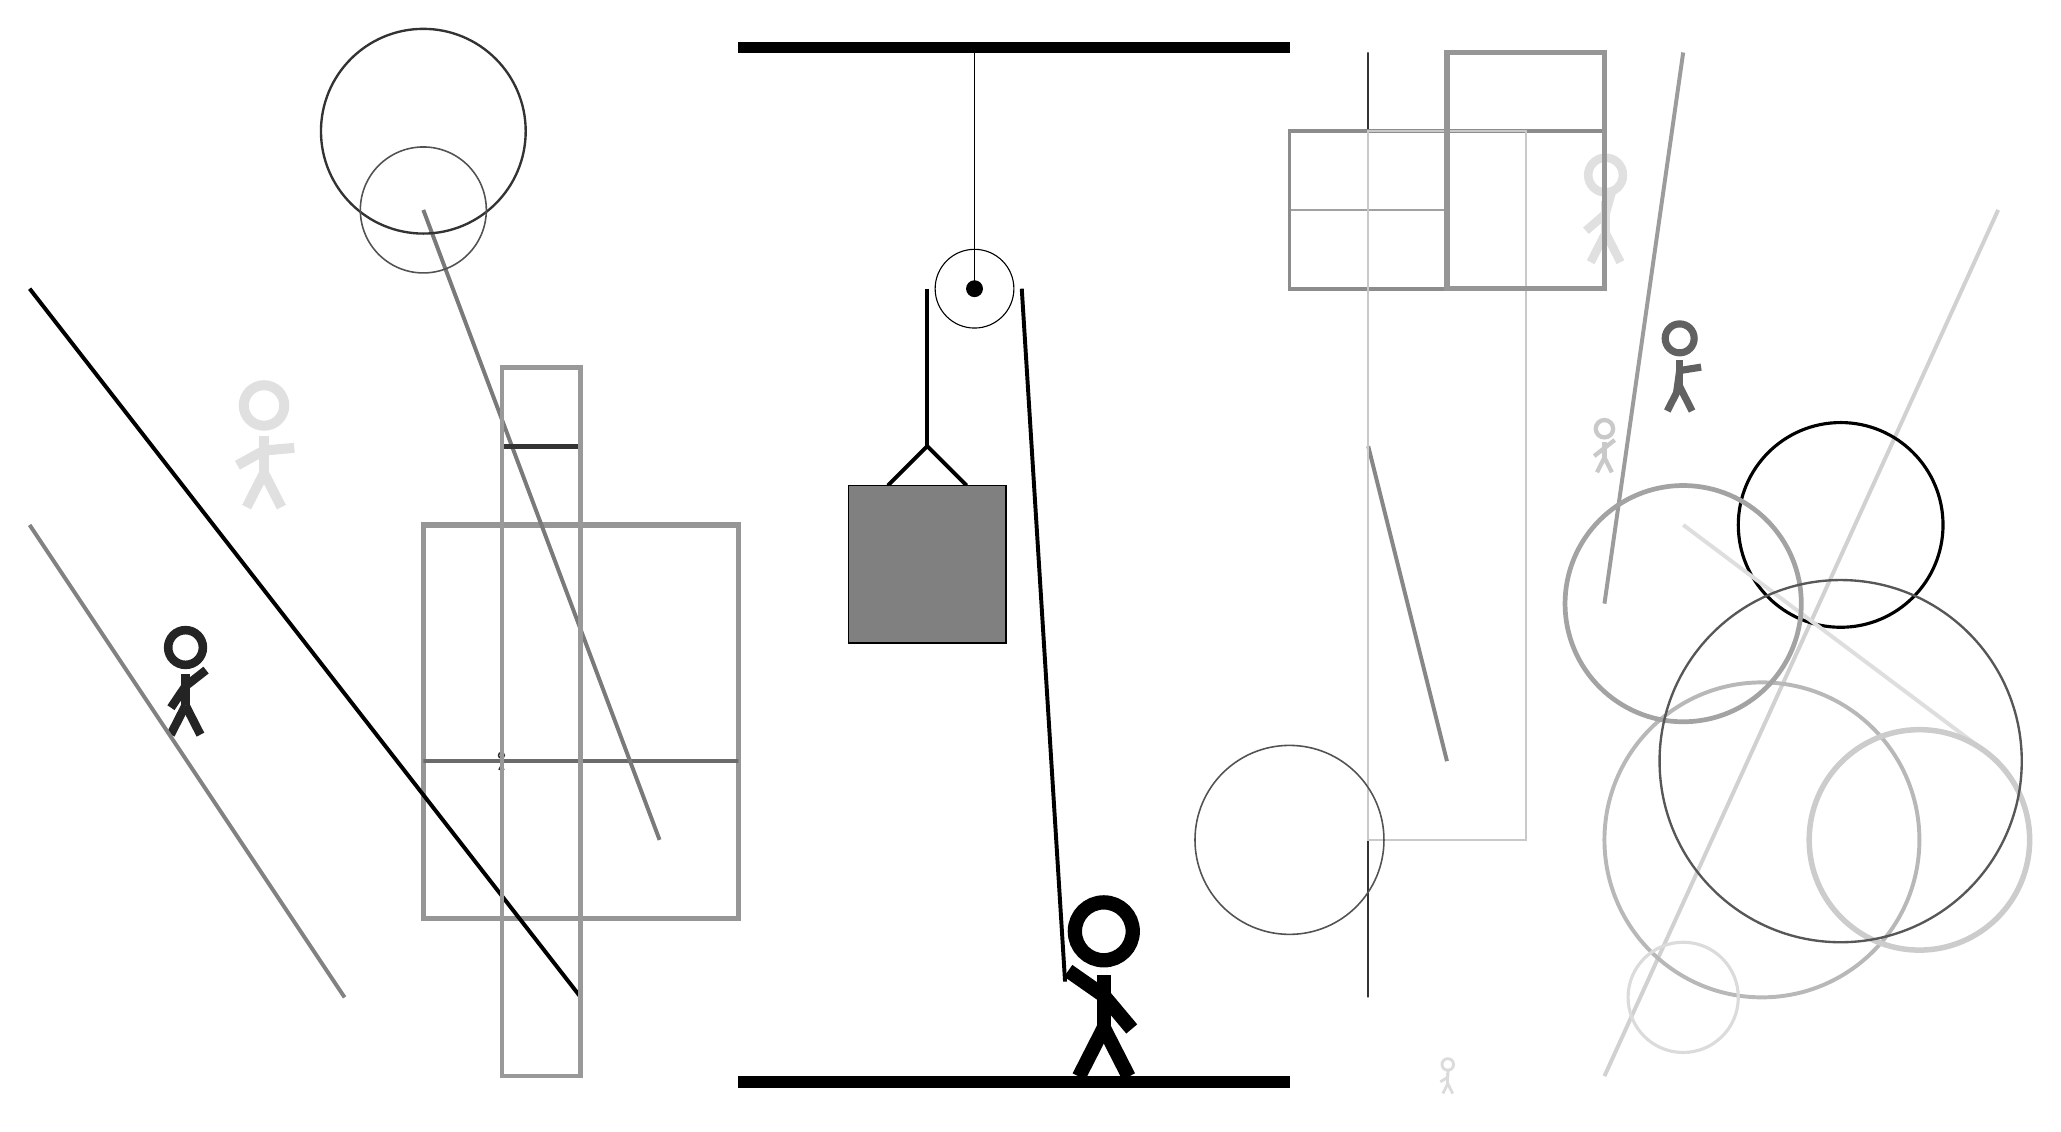
\begin{tikzpicture}
		%%%%% START %%%%%
		
		\draw[fill=black] (-2, 10) rectangle (5, 10.125);
		
		\draw[line width=0.5mm, color=black!47](7, 1) -- (6, 5);
		
		\node[line width=0.6mm, color=black!12] at (9, 8) {\Strichmaxerl[6][41][74]};
		\node[line width=0.6mm, color=black!62] at (10, 6) {\Strichmaxerl[5][82][9]};
		\node[line width=0.4mm, color=black!84] at (-5, 1) {\Strichmaxerl[1][81][12]};
		
		\draw[line width=0.7mm, color=black!41] (-2, -1) rectangle (-6, 4);
		\draw[line width=0.5mm, color=black!58] (-2, 1) rectangle (-6, 1);
		\node[line width=0.5mm, color=black!14] at (7, -3) {\Strichmaxerl[2][31][87]};
		\node[line width=0.2mm, color=black!12] at (-8, 5) {\Strichmaxerl[7][29][5]};
		\draw[line width=0.3mm, color=black!80] (6, -2) rectangle (6, 10);
		
		\draw[line width=0.5mm, color=black!52](-3, 0) -- (-6, 8);
		\draw[line width=0.5mm, color=black!18](9, -3) -- (14, 8);
		
		\draw[line width=0.2mm, color=black!37] (7, 8) rectangle (5, 7);
		\draw[line width=0.5mm, color=black!45] (5, 9) rectangle (9, 7);
		
		\draw [line width=0.5mm, color=black!28](11, 0) circle (2.0);
		\draw [line width=0.4mm, color=black!100](12, 4) circle (1.3);
		\draw [line width=0.3mm, color=black!80](-6, 9) circle (1.3);
		\draw[line width=0.5mm, color=black!39](9, 3) -- (10, 10);
		
		\draw[line width=0.6mm, color=black!80] (-4, -3) rectangle (-5, 5);
		\draw[line width=0.3mm, color=black!21] (6, 0) rectangle (8, 9);
		\draw[line width=0.5mm, color=black!13](10, 4) -- (14, 1);
		\draw[line width=0.5mm, color=black!100](-4, -2) -- (-11, 7);
		
		\node[line width=0.4mm, color=black!21] at (9, 5) {\Strichmaxerl[3][38][38]};
		
		\node[line width=0.4mm, color=black!86] at (-9, 2) {\Strichmaxerl[6][56][38]};
		\draw [line width=0.6mm, color=black!36](10, 3) circle (1.5);
		\draw [line width=0.2mm, color=black!68](5, 0) circle (1.2);
		
		\draw [line width=0.4mm, color=black!14](10, -2) circle (0.7);
		\draw [line width=0.2mm, color=black!68](-6, 8) circle (0.8);
		\draw[line width=0.6mm, color=black!40] (-4, -3) rectangle (-5, 6);
		\draw[line width=0.7mm, color=black!41] (7, 7) rectangle (9, 10);
		
		\draw [line width=0.7mm, color=black!20](13, 0) circle (1.4);
		\draw[line width=0.5mm, color=black!49](-7, -2) -- (-11, 4);
		\draw [line width=0.3mm, color=black!66](12, 1) circle (2.3);
		
		\draw (1, 7) circle (0.5);
		\draw[fill=black] (1, 7) circle (0.1);
		\draw (1, 10) -- (1, 7);
		
		\draw[line width=0.5mm] (-0.1, 4.5) -- (0.4, 5.0) -- (0.9, 4.5);
		\draw[fill=black!50] (-0.6, 4.5) rectangle (1.4, 2.5);
		
		\draw[line width=0.5mm] (0.4, 7) -- (0.4, 5.0);
		\centerarc[line width=0.5mm](1, 7)(0:180:0.6);
		\draw[line width=0.5mm](1.6, 7) -- (2.15, -1.8);
		
		\node at (2.6, -1.9) {\Strichmaxerl[10][-35][-50]};
		
		\draw[fill=black] (-2, -3) rectangle (5, -3.15);
		
		%%%%% END %%%%%
	\end{tikzpicture}
\end{document}